\documentclass[11pt]{article}
\usepackage[margin=0.8in]{geometry}            % See geometry.pdf to learn the layout options. There are lots.
\geometry{letterpaper}                                  % ... or a4paper or a5paper or ... 
%\geometry{landscape}                           % Activate for rotated page geometry
%\usepackage[parfill]{parskip}                  % Activate to begin paragraphs with an empty line rather than an indent
\usepackage{graphicx}                                         
\usepackage{amssymb}
\usepackage{upquote}
\usepackage{enumerate}
\usepackage{subcaption} % for side-by-side figures
\usepackage{wrapfig} % for wrapping figures around text
\usepackage{lipsum} % for wrapping figures around text
\usepackage{float}
%-----------------------------------------------------------------------------
% Special-purpose color definitions (dark enough to print OK in black and white)
\usepackage{color}
% A few colors to replace the defaults for certain link types
\definecolor{orange}{cmyk}{0,0.4,0.8,0.2}
\definecolor{darkorange}{rgb}{.71,0.21,0.01}
\definecolor{darkgreen}{rgb}{.12,.54,.11}
%-----------------------------------------------------------------------------
% The hyperref package gives us a pdf with properly built
% internal navigation ('pdf bookmarks' for the table of contents,
% internal cross-reference links, web links for URLs, etc.)
\usepackage{hyperref}
\hypersetup{pdftex, % needed for pdflatex
  breaklinks=true, % so long urls are correctly broken across lines
  colorlinks=true,
  urlcolor=blue,
  linkcolor=darkorange,
  citecolor=darkgreen
}


\title{Cloud Data}

\author{
  Zizhuo Tian (SID: 2793557)
}


\begin{document}
\maketitle


\section{Data Collection and Exploration}
\subsection{Summary of the Paper} 

\quad\ \ The goal of the study [1] is to build an operational cloud detection algorithm on massive MISR(Multiangle imaging spectroradiometer) data with high efficiency and accuracy. Unlike existing MISR algorithms, the proposed algorithms detect cloud-free pixels instead of cloudy or snowy pixels. The data used in this study were orbits of path 26 MISR data, which has rich features across the Arctic Ocean to Greenland. The most important step is feature engineering to produce representative new features to summarize physical properties of MISR images: CORR as the correlation of the same scene from different directions; SDan as standard deviation of nadir camera pixel values across a scene; DNAI as normalized difference angular index that characterizes the changes in scene with changes in view directions. Two algorithms were invented based on the three new features. Enhanced Linear Correlation Matching (ELCM) algorithm uses CORR and SDan thresholds to label data units sequentially. The second algorithm ELCM-QDA uses labels from the ELCM algorithm to train Fisher's quadratic discriminant analysis to produce probability labels. The study proposed an efficient cloud detection algorithm on MISR data, and it demonstrated the power of statistical approaches to solve complex scientific problems. The fruit of the research could also contribute to future global climate models.


\subsection{Data Summary}

\quad\ \  There are three images data tables in the data set, and for each data table, I draw the coordinate distribution map of the weather. Regions of different colors in the image represent different weather labels. From the distribution profile of the colors, there is no obvious pattern in the distribution of the weather.

The label ratios differ by each image. The majority of labels are not cloud, and the minority is cloud. The big portion of data is unlabeled Based on the plots for the three images above, a clear boundary between cloud (label 1) and not cloud (label -1) is formed by unlabeled data. Given the words from the paper that experts leave uncertain data points with no label because of low confidence, I can assume that cloud and non-cloud data are separable and regions with the same label are mostly connected. Those unlabeled data may also have similar qualities which can not be differentiated from either cloud or non-cloud. Therefore, the x axis and y axis can not be used to separate the data, they may work with other features or project the data to other dimensions.
\begin{figure}[H]
  \centering
  \begin{subfigure}{.5\textwidth}
    \centering
      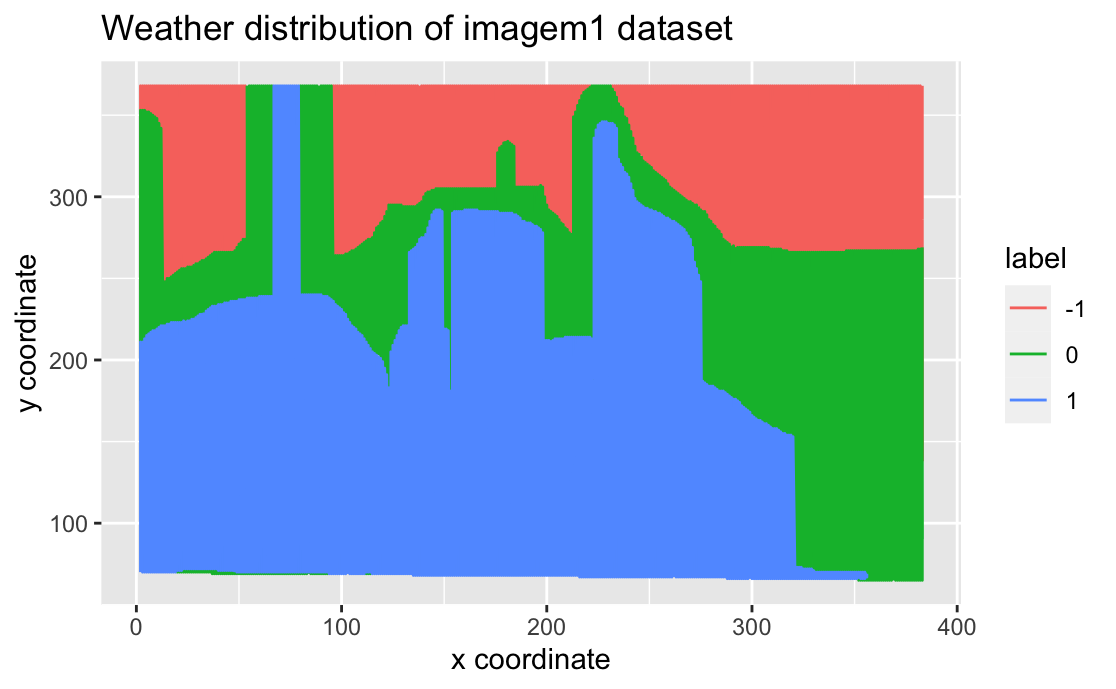
\includegraphics[width=1\textwidth, height=0.6\textwidth]{../figures/figure1.png}    
  \end{subfigure}%  
  \begin{subfigure}{.5\textwidth}
    \centering
      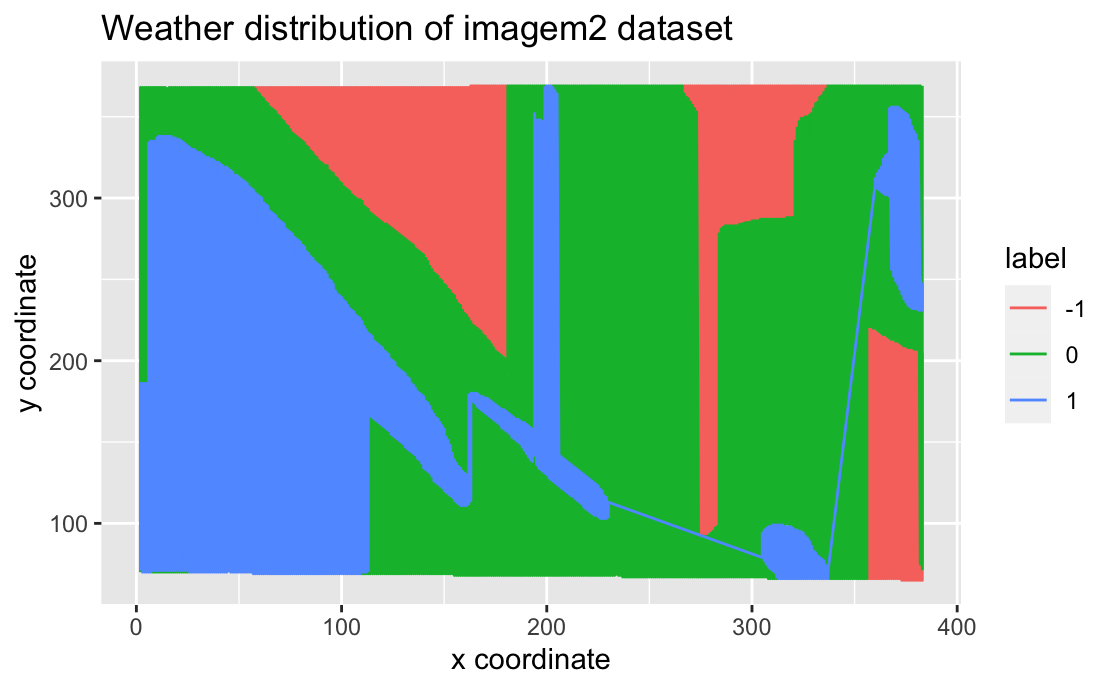
\includegraphics[width=1\textwidth, height=0.6\textwidth]{../figures/figure2.png}
  \end{subfigure}%
  
  \begin{subfigure}{.5\textwidth}
    \centering
      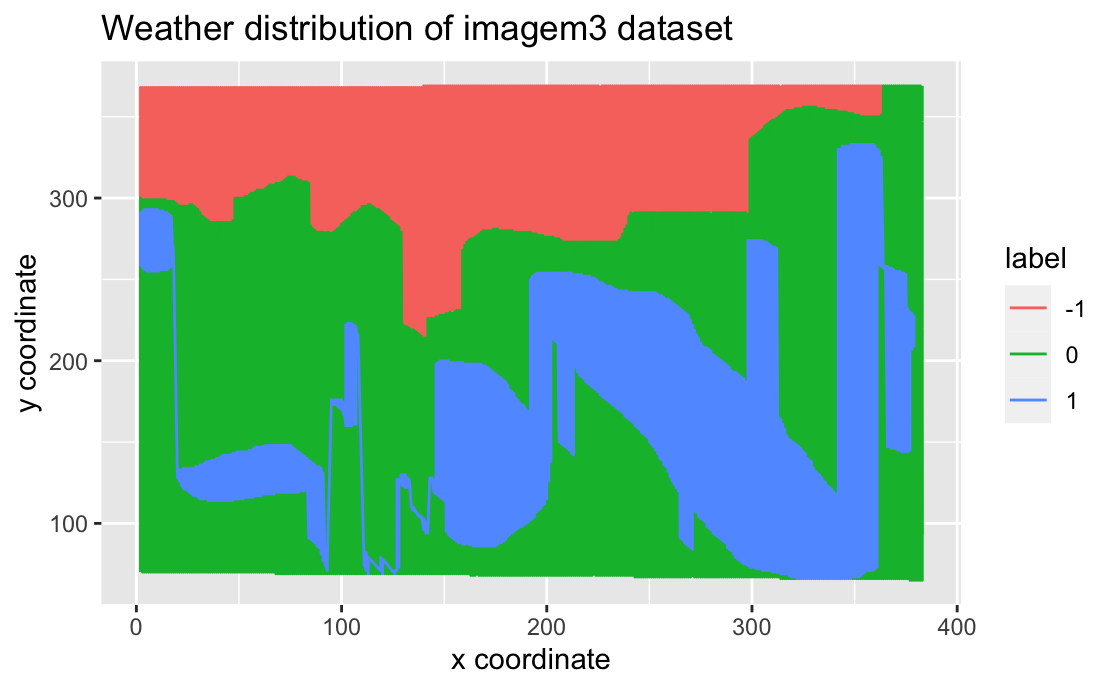
\includegraphics[width=1\textwidth, height=0.6\textwidth]{../figures/figure3.png}
  \end{subfigure}
  \caption{Image of Three Dataset}
\end{figure}

\bigskip

In addition, we count the proportions of different weather labels for the three images data, and I can find that the weather label distributions of the three images are not consistent. Therefore I do not consider the data samples to be independent and identically distributed.
\begin{table}[htbp]
\centering
	\begin{tabular}{|c|c|c|c|}  
		\hline  
		& & & \\[-8pt]  
		Expert label&image 1&image 2&image 3 \\ 
		\hline
		& & & \\[-8pt] 
		-1&37.25$\%$&43.78$\%$&29.29$\%$ \\
		\hline
		& & & \\[-8pt] 
		0&28.64$\%$&38.46$\%$&52.27$\%$ \\
		\hline
		& & & \\[-8pt] 
		1&34.11$\%$&17.77$\%$&18.44$\%$ \\
		\hline
		& & & \\[-8pt] 
		Total&100.00$\%$&100.00$\%$&100.00$\%$ \\
		\hline
	\end{tabular}
\end{table}

\subsection{Quantitative EDA}

\quad\ \  I calculate the correlation coefficient between different features, and its correlation matrix is shown in the figure below. The red asterisk in the upper right corner of the correlation coefficient indicates that the correlation between the two variables is significant at the 0.01 significance level. According to the correlation coefficient, there is a high correlation among the variables \textbf{DF}, \textbf{CF}, \textbf{BF}, \textbf{AN}, \textbf{AF}. However, there is a weak negative correlation with other variables.

\begin{figure}[H]
  \centering
      \includegraphics[width=0.8\textwidth, height=0.5\textwidth]{../figures/coefficient.png}     
   \caption{Correlation Coefficient between Features}
\end{figure}

In addition, there are significant differences in the distribution of different weather labels on \textbf{CORR}, \textbf{NDAI}, and \textbf{SD} features. For example, cloud cases are significantly higher than not cloud cases in these three characteristics. It means that when a sample has a relatively large value on \textbf{CORR}, \textbf{NDAI}, and \textbf{SD}, the probability of being predicted as cloud will be higher.

\begin{figure}[h]
  \centering
      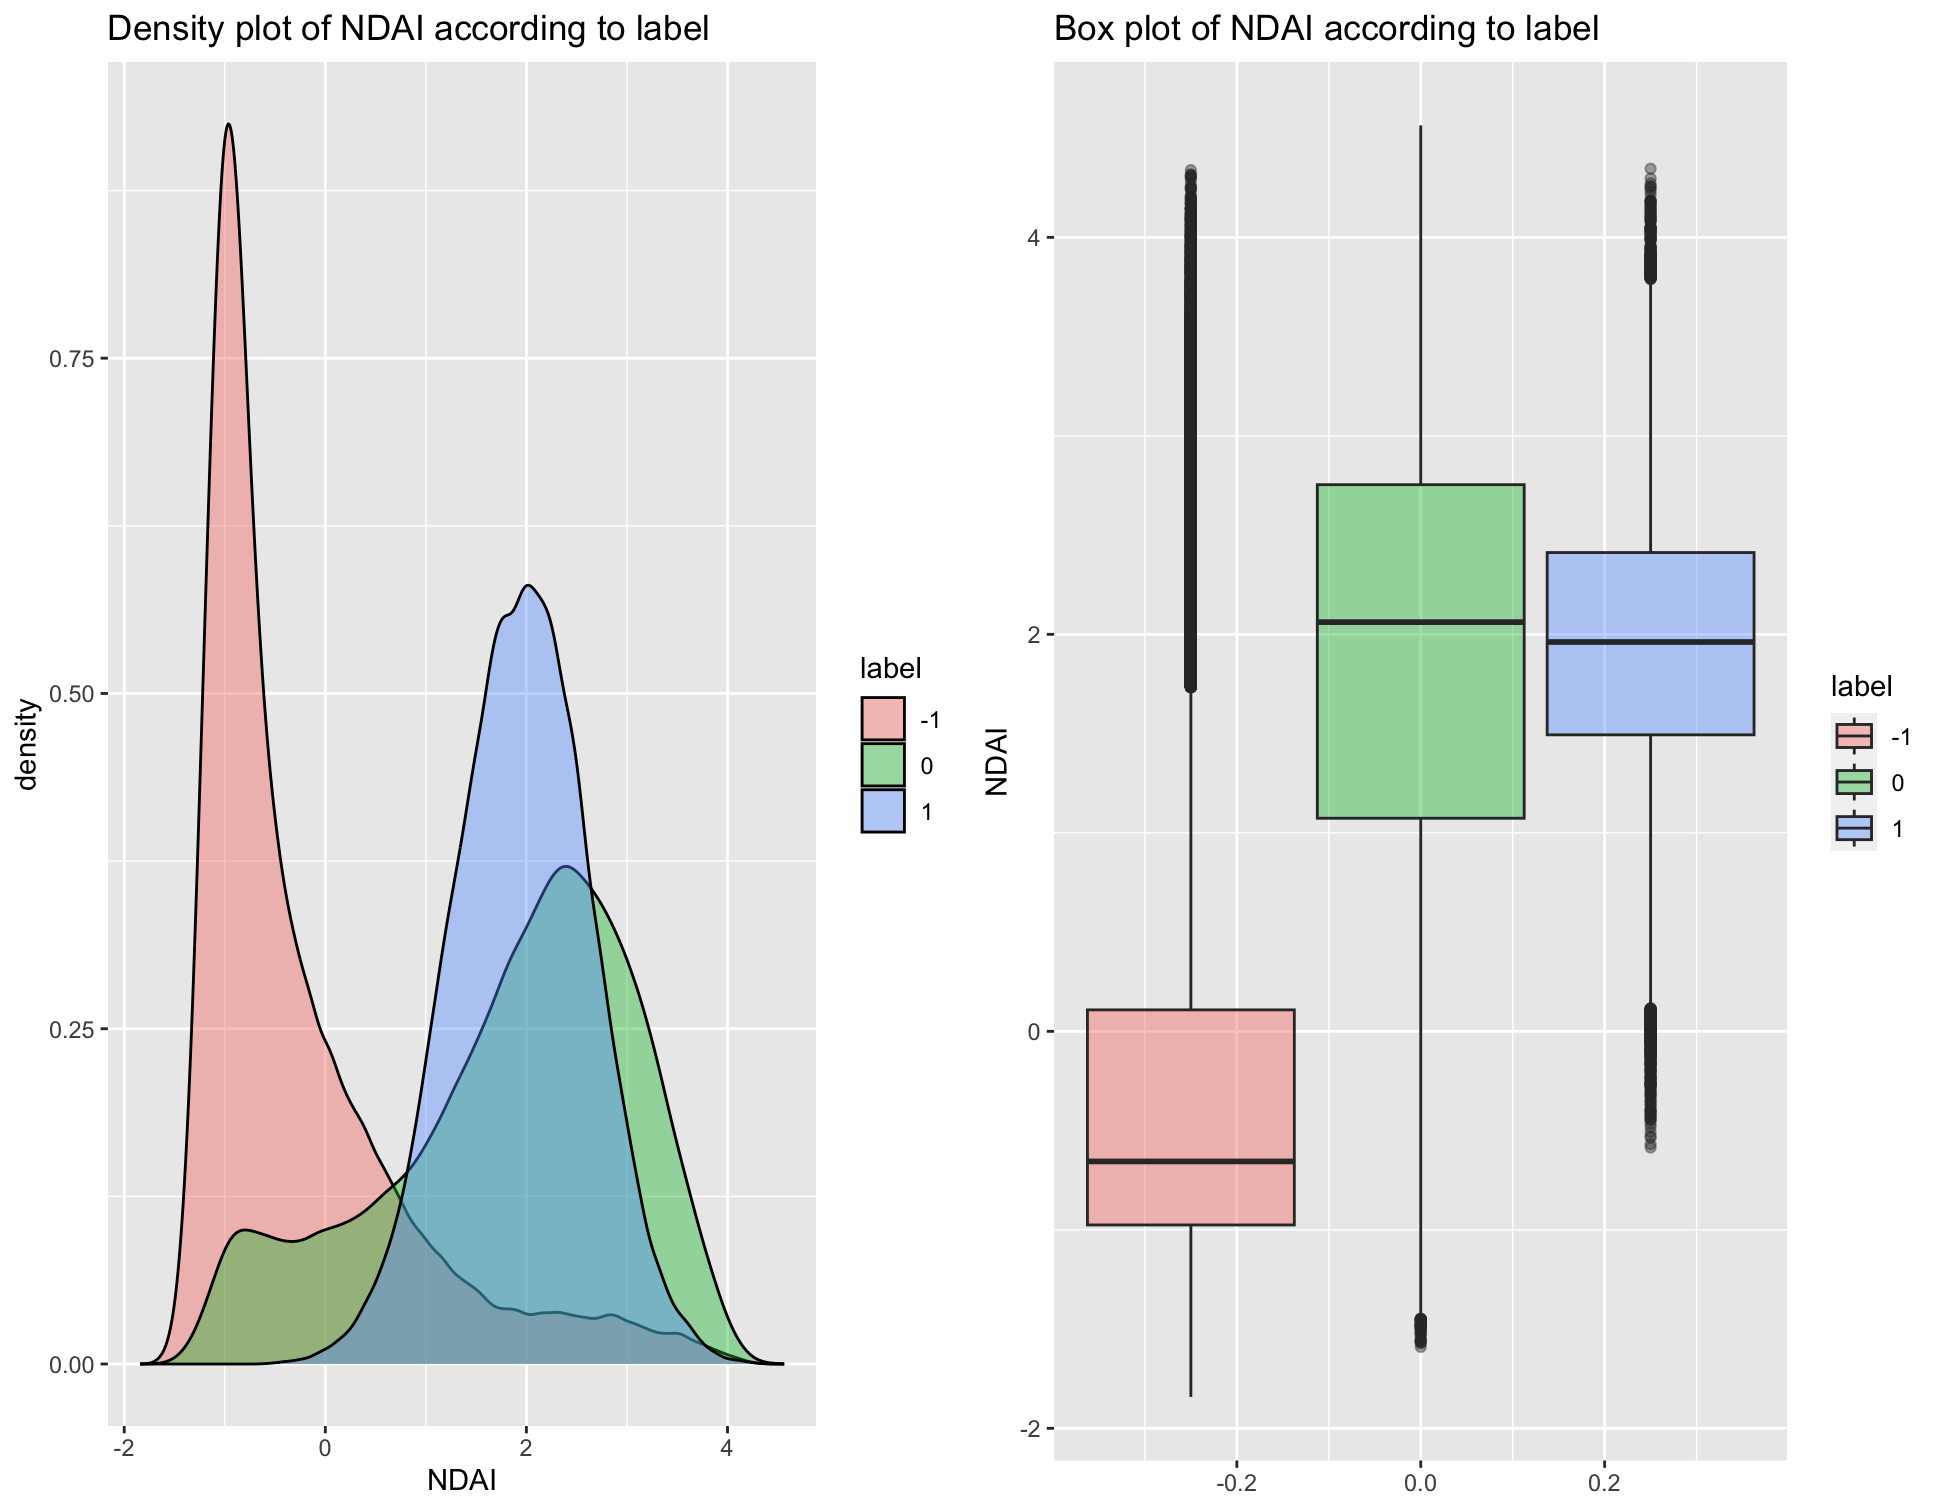
\includegraphics[width=0.8\textwidth, height=0.5\textwidth]{../figures/NDAI_dis.png}
  \caption{NDAI Distribution}
\end{figure}

\begin{figure}[H]
  \centering
      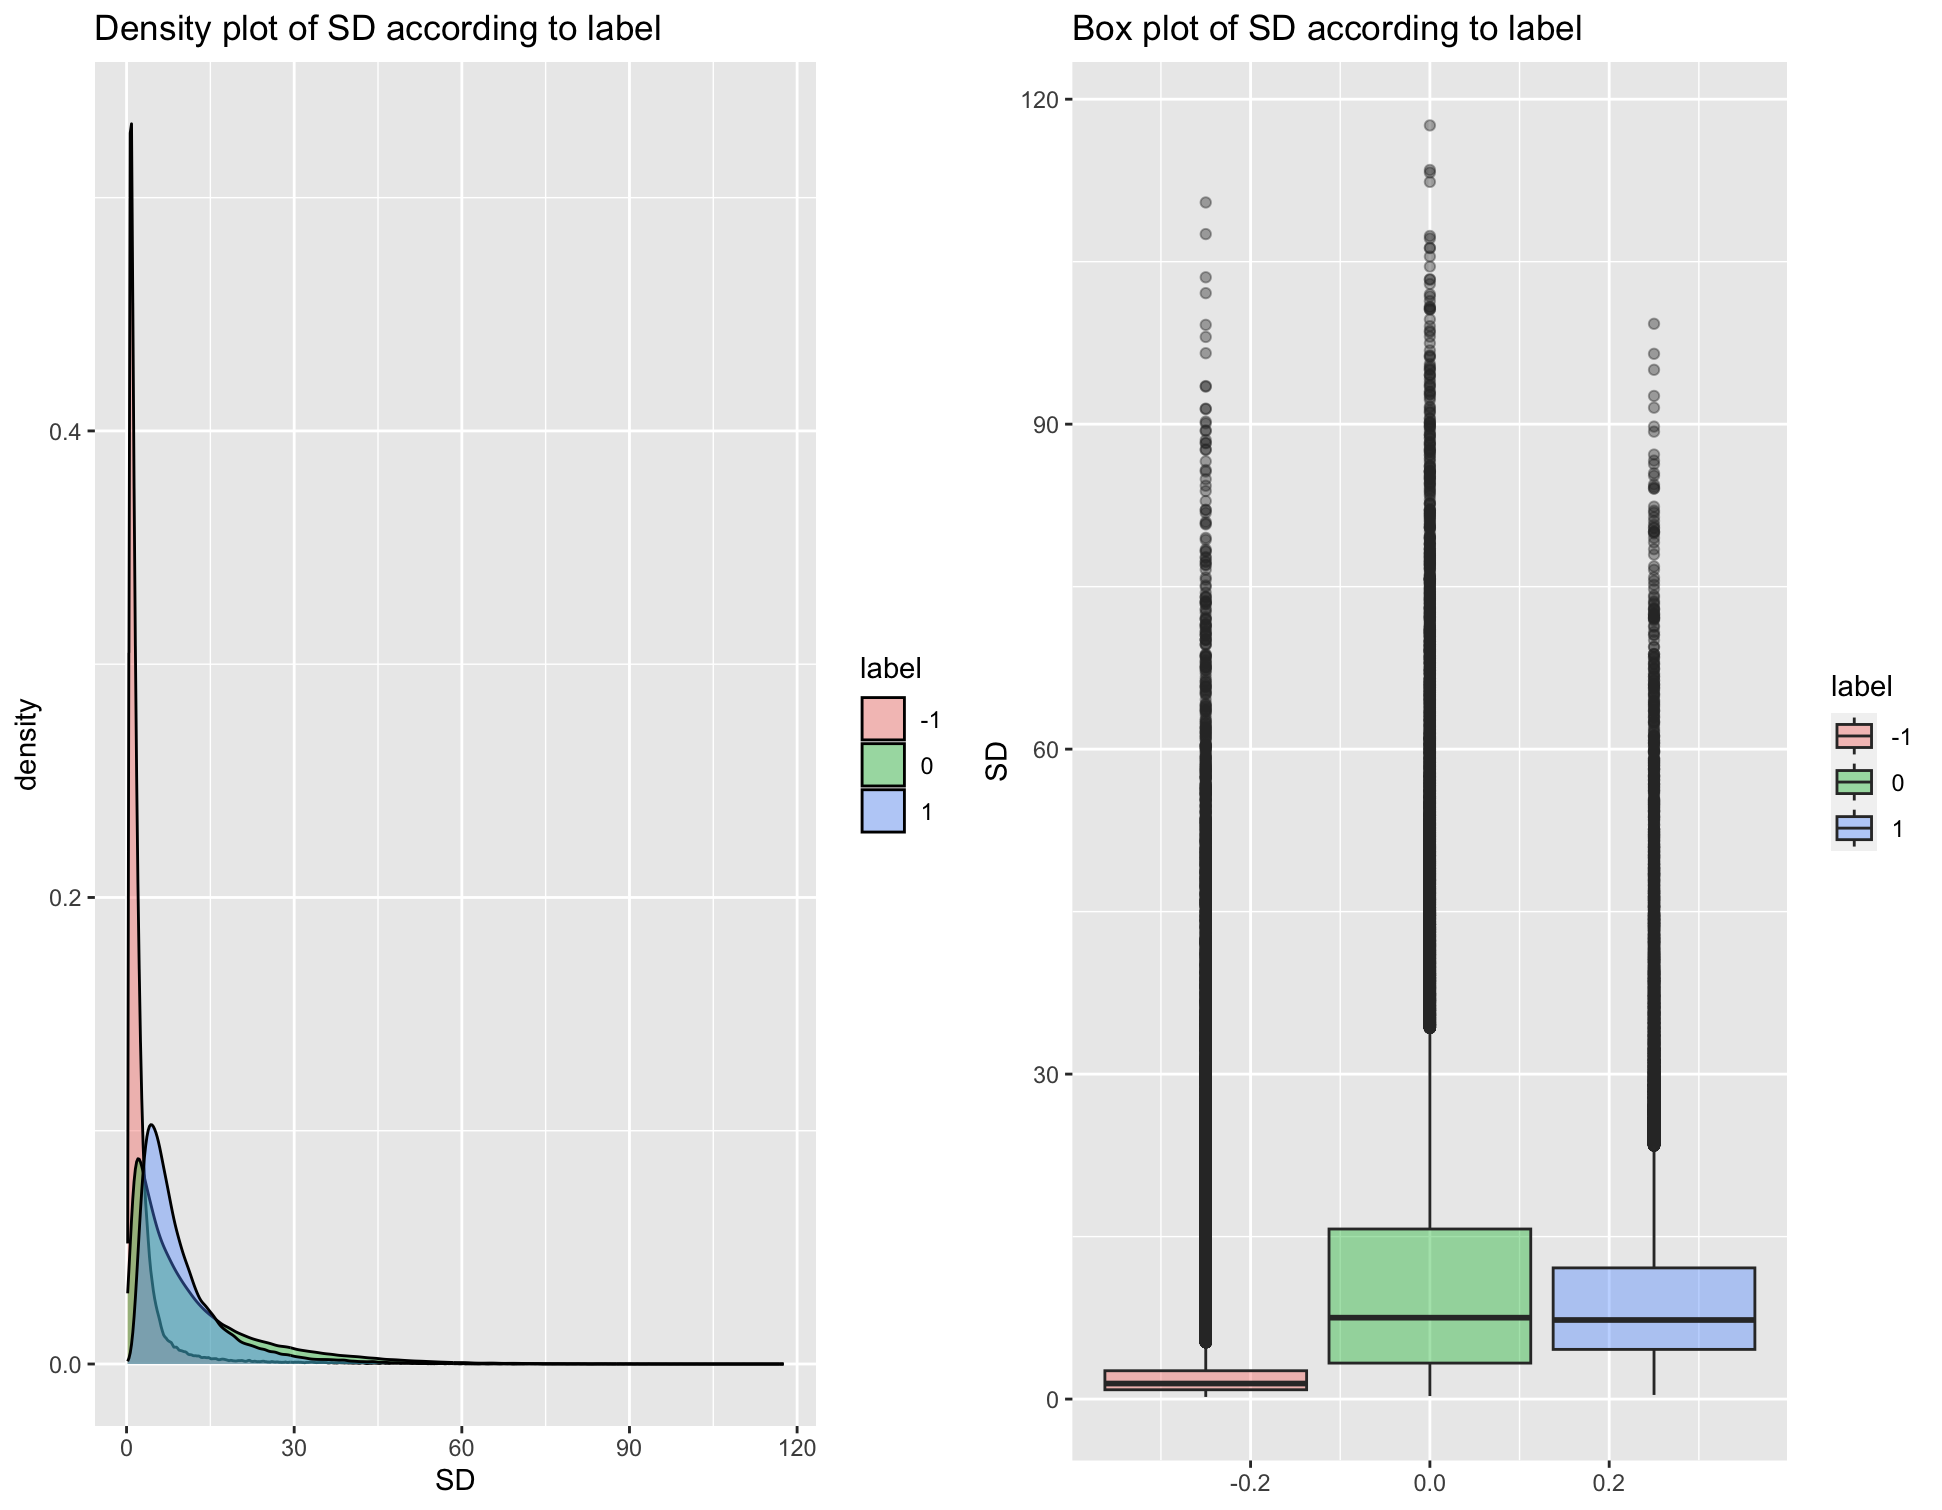
\includegraphics[width=0.8\textwidth, height=0.5\textwidth]{../figures/SD_dis.png}
    \caption{SD Distribution}
  \end{figure}
  
 \begin{figure}[H]
  \centering 
      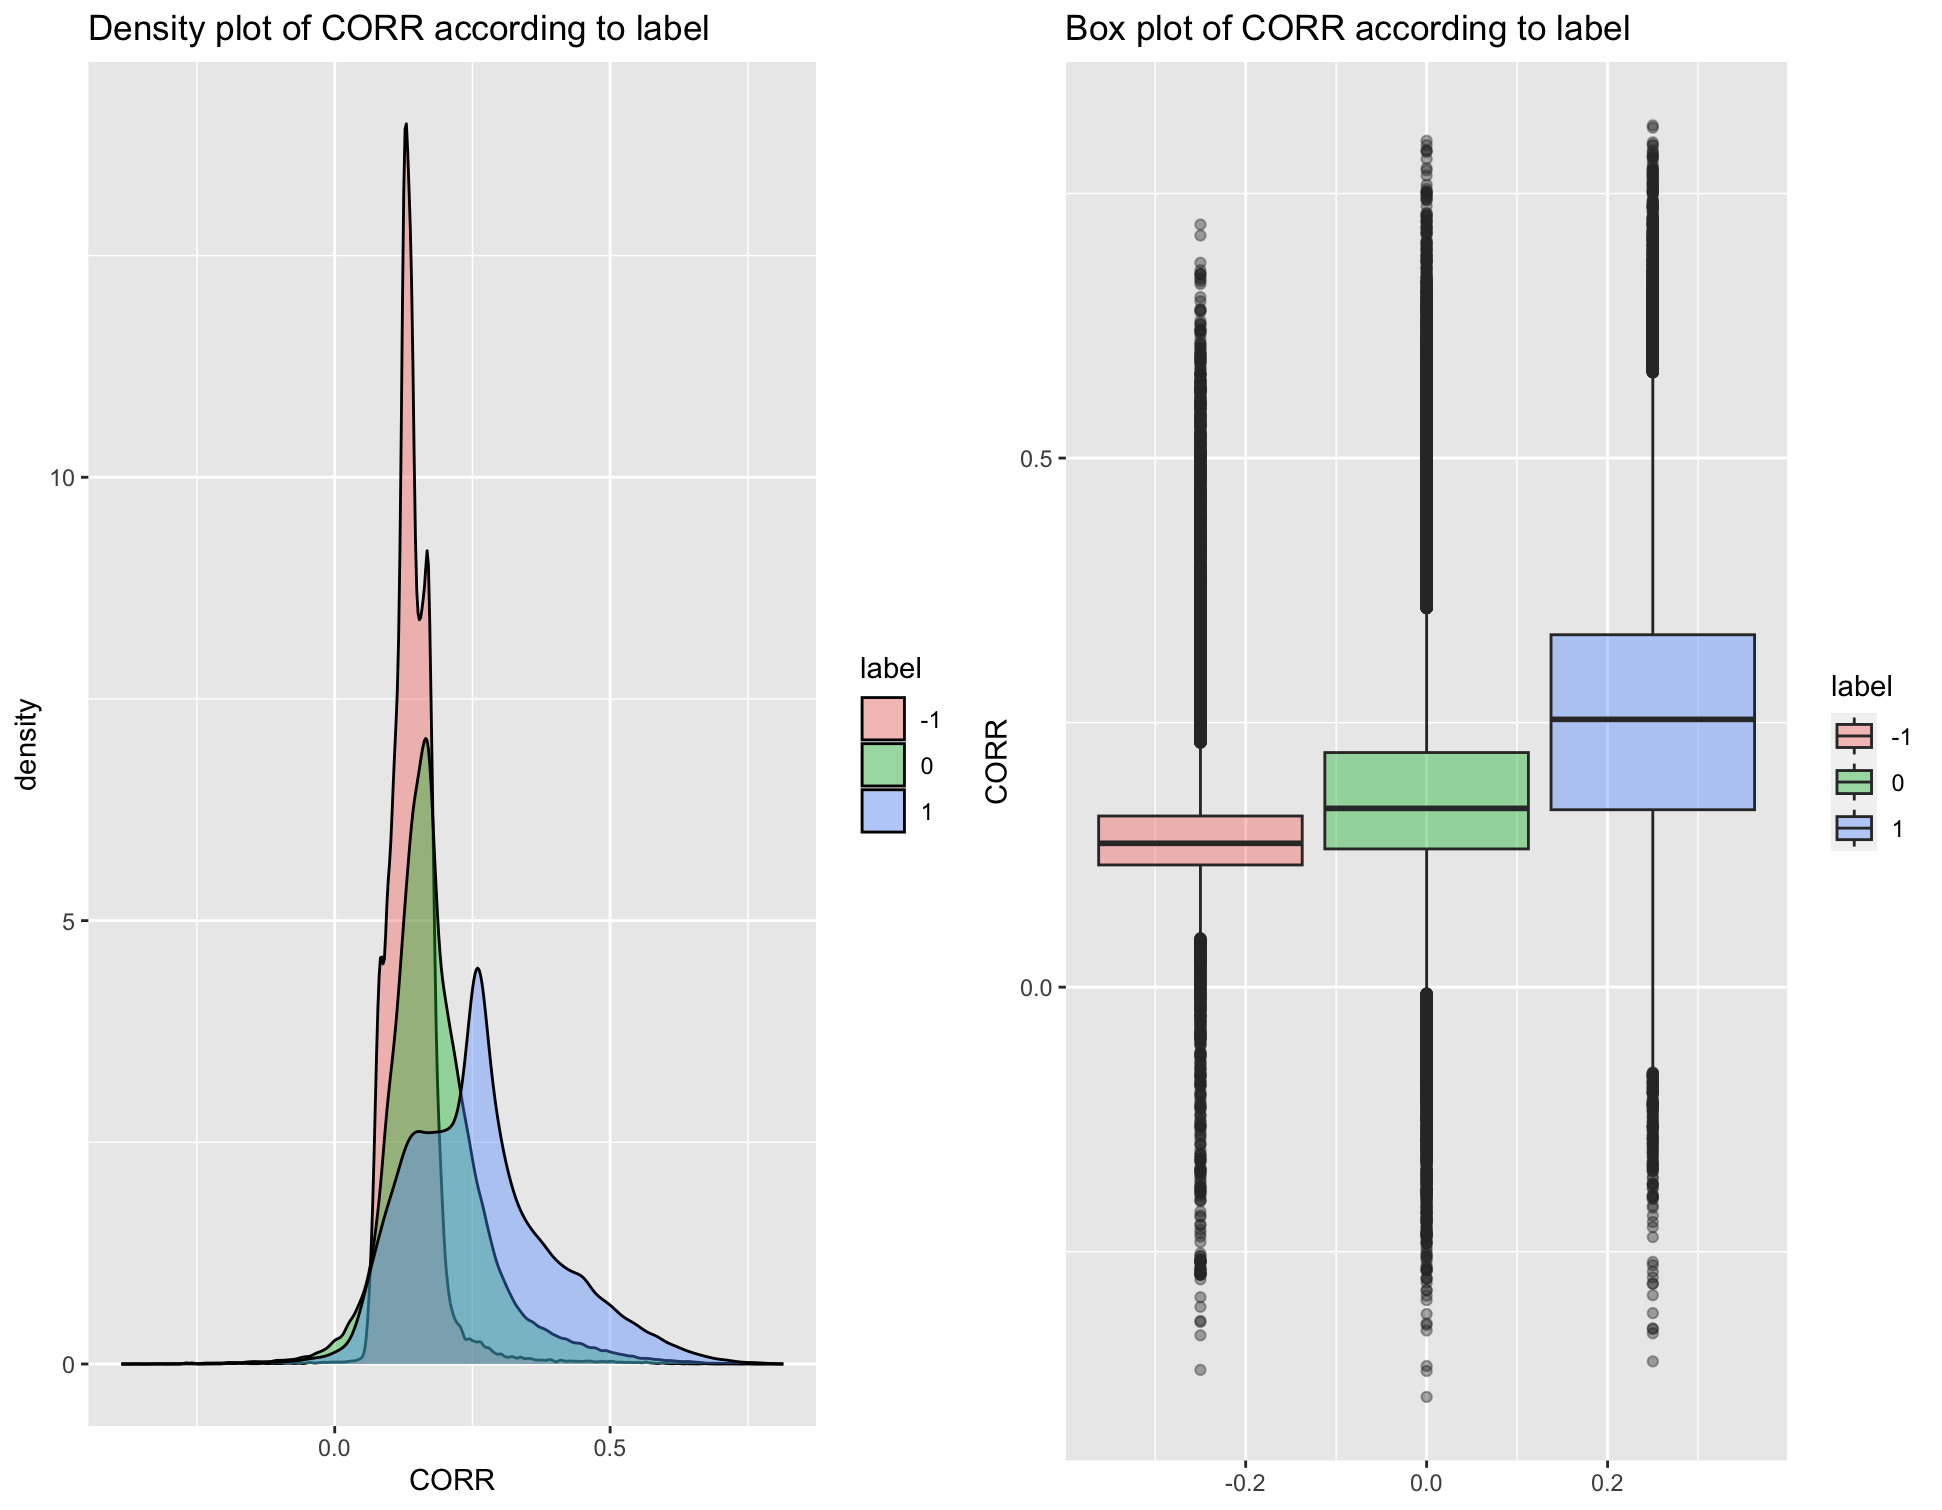
\includegraphics[width=0.8\textwidth, height=0.5\textwidth]{../figures/CORR_dis.png}
          \caption{CORR Distribution}
\end{figure}

\newpage
\section{Preparation}
\subsection{Use Two Non-trivial Methods to Split the Data} 

The standard data preparation process to both splitting methods are:
\begin{enumerate}[1.]
\item Shuffle the whole dataset by resampling.
\item Remove unlabeled data since I'm doing supervised learning with cloud and non-cloud only.
\item Split the data to training, validation and testing index as ratios of 0.8. 0.1, 0.1.
\item Filter data by index derived from step 2 and apply standard normalization to feature columns because value range can affect the overall euclidean distance for any dissimilarity based algorithms like KNN and clustering algorithms. 
\end{enumerate}
\begin{itemize}
  \item \textbf{Method 1 -  Split the data according to label distribution}
 
 After removing unlabeled data, the label distribution of cloud and non-cloud is still imbalanced. Therefore, the first method is to split the data into training, validation and testing sets while retaining label distribution. In order to retain the label ratio of 0.611 for non-cloud and 0.389 for cloud, the \texttt{createPartition} function was used to split the data with shuffle before every split. 
 
 \item \textbf{Method 2 - Stratified sampling to reduce variance}
 
Imbalanced label distribution would require a modified loss function for most machine learning algorithms and affect model accuracy. With stratified sampling, the label distribution has been resampled to 0.5 versus 0.5. The difference between the two methods is the label distribution after resampling. Method 2 change the label ratio to half-half instead of retaining the original $60\%$ versus $40\%$
\end{itemize}

\subsection{Accuracy of Trivial Classifier}

I build a very simple classification model, which sets all labels to -1 (not cloud) on the validation set and on the test set. Although this classifier has no predictive value, I can use it as a trivial classifier, which provides a baseline to ensure that the classification problems at hand is not trivial. For the two sampling methods, the trivial classifier on the validation set and test set the classification accuracy is as follows:
\begin{table}[htbp]
\centering
	\begin{tabular}{|c|c|c|}  
		\hline  
		& & \\[-8pt]  
		Accuracy&Random Sampling&Stratified Sampling \\ 
		\hline
		& & \\[-8pt] 
		Validation Set&0.608&0.497 \\
		\hline
		& & \\[-8pt] 
		Test Set&0.614&0.481 \\
		\hline
	\end{tabular}
\end{table}

\subsection{Suggest Three of the Best Features}

When the question comes to ranking features based on importance, random forest could be in great use for this problem because it reports decrease of node impurity when the variable has been removed. Features were ranked when splitting to nodes in multiple trees. Based on Gini importance, \textbf{NDAI}, \textbf{y}, \textbf{AN} are ranked the top three features.
\begin{figure}[H]
  \centering
      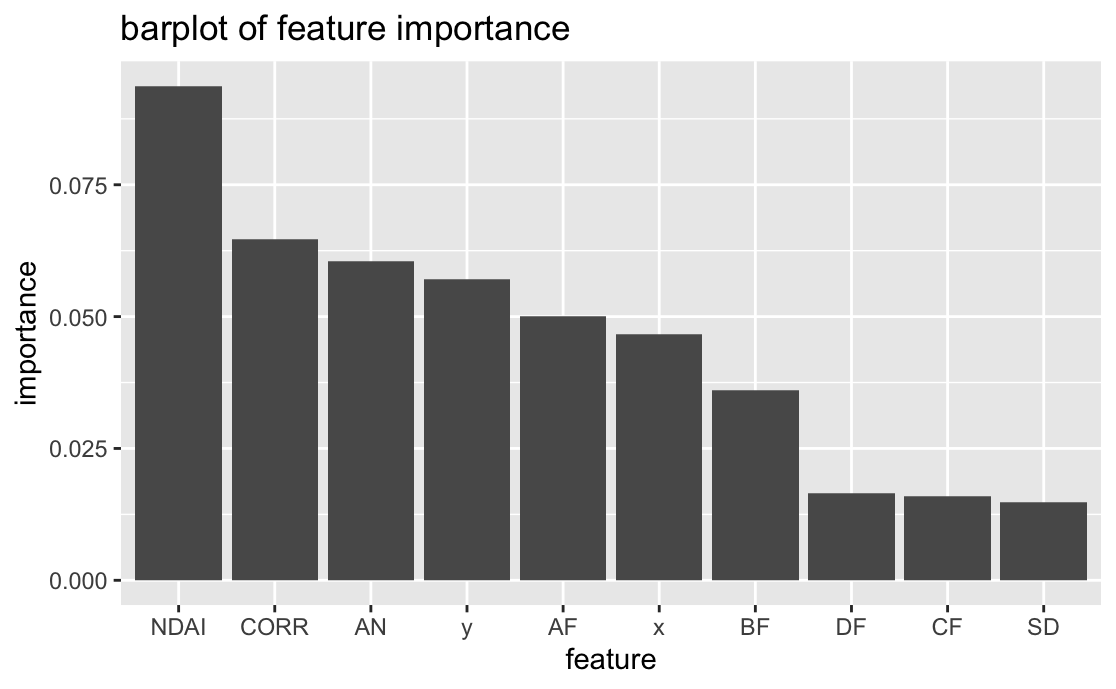
\includegraphics[width=0.8\textwidth, height=0.5\textwidth]{../figures/ranking.png}
  \caption{Importance Ranking Barplot}
\end{figure}

\section{Modelling}

\quad\ \ This is a binary classification task. I consider 4 classification models: Logistic Regression, Decision Tree, Random Forest and Support Vector Machine (SVM). 

For each classification model, I use 5-fold cross-validation to train the model. Since CV does not have a validation set, I merge the training and validation set to fit CV model. Also, I used two sampling methods earlier, so for each model, I train two sampling samples separately, and calculate the classification accuracy for each fold, as well as the classification accuracy on the test set.
\bigskip

\begin{enumerate}[-]
  \item For the random sampling method, the classification accuracy of the four models is as follows:
\\
\begin{table}[htbp]
\centering
	\begin{tabular}{|c|c|c|c|c|}  
		\hline  
		& & & &\\[-8pt]  
		Model&Logistic Regression&Decision Tree& Random Forest & SVM \\ 
		\hline
		& & & &\\[-8pt] 
		Fold 1 &0.8955 &0.9884 &0.9758 &0.9750 \\
		\hline
		& & & &\\[-8pt] 
		Fold 2& 0.8955 & 0.9876 &0.9778 &0.9746 \\
		\hline
		& & & &\\[-8pt] 
		Fold 3& 0.8943 &0.9878 &0.9787 &0.9737 \\
		\hline
		& & & &\\[-8pt] 
		Fold 4& 0.8951 &0.9884 &0.9818 &0.9720 \\
		\hline
		& & & &\\[-8pt] 
		Fold 5& 0.8946 &0.9873 &0.9778 &0.9735 \\
		\hline
		& & & &\\[-8pt] 
		Cross-validation Average&0.8915 &0.9879 &0.9784 &0.9738 \\
		\hline
		& & & &\\[-8pt] 
		Testing Accuracy&0.8915 &0.9865 &0.9708 &0.9688 \\
		\hline
	\end{tabular}
\end{table}
\\
\\
\\
\item For the stratified sampling method, the classification accuracy of the four models is as follows:
\\
\begin{table}[htbp]
\centering
	\begin{tabular}{|c|c|c|c|c|}  
		\hline  
		& & & &\\[-8pt]  
		Model&Logistic Regression&Decision Tree& Random Forest & SVM \\ 
		\hline
		& & & &\\[-8pt] 
		Fold 1 &0.9031 &0.9644 &0.9708 &0.9708  \\
		\hline
		& & & &\\[-8pt] 
		Fold 2& 0.9017 &0.9639 &0.9742 &0.9711 \\
		\hline
		& & & &\\[-8pt] 
		Fold 3& 0.9017 &0.9642 &0.9694 &0.9739  \\
		\hline
		& & & &\\[-8pt] 
		Fold 4& 0.9039&0.9672 &0.9720 &0.9728  \\
		\hline
		& & & &\\[-8pt] 
		Fold 5& 0.8986 &0.9625 &0.9758 &0.9658  \\
		\hline
		& & & &\\[-8pt] 
		Cross-validation Average&0.9018 &0.9644 &0.9724 &0.9709  \\
		\hline
		& & & &\\[-8pt] 
		Testing Accuracy&0.9050 &0.9590 &0.9735 &0.9688  \\
		\hline
	\end{tabular}
\end{table}
\end{enumerate}

\begin{itemize}
\item The test set ROC of the logistic regression model in random sampling samples and stratified sampling samples are as follows:
\begin{figure}[H]
  \centering
  \begin{subfigure}{.5\textwidth}
    \centering
      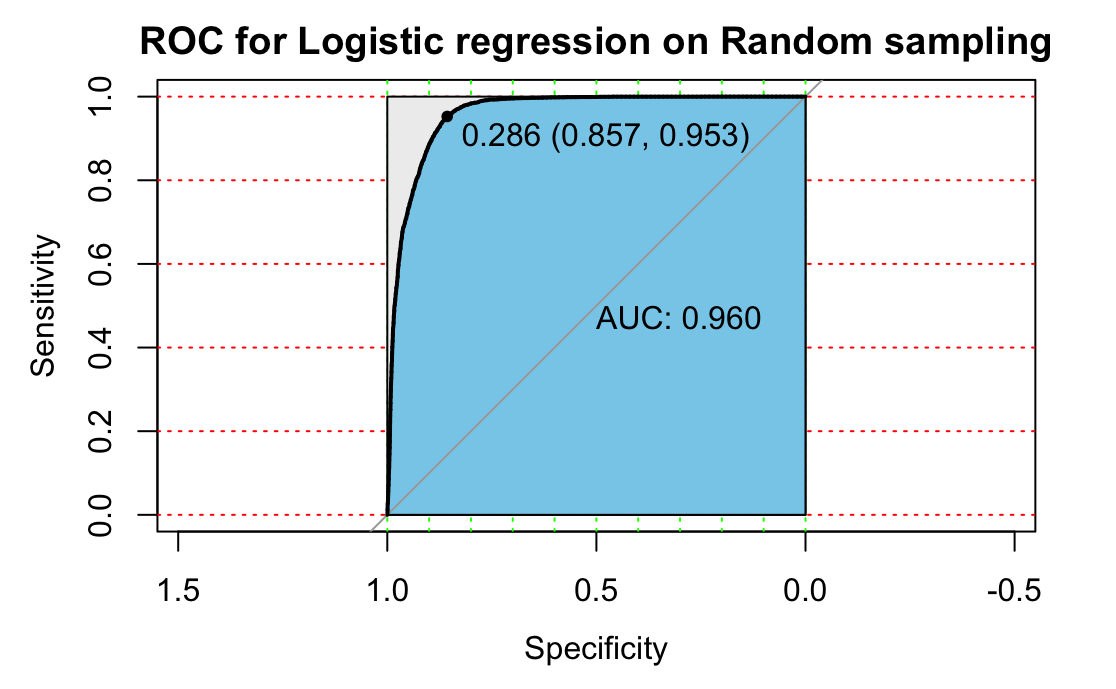
\includegraphics[width=1\textwidth, height=0.65\textwidth]{../figures/ROC_LR_random.png}    
  \end{subfigure}%  
  \begin{subfigure}{.5\textwidth}
    \centering
      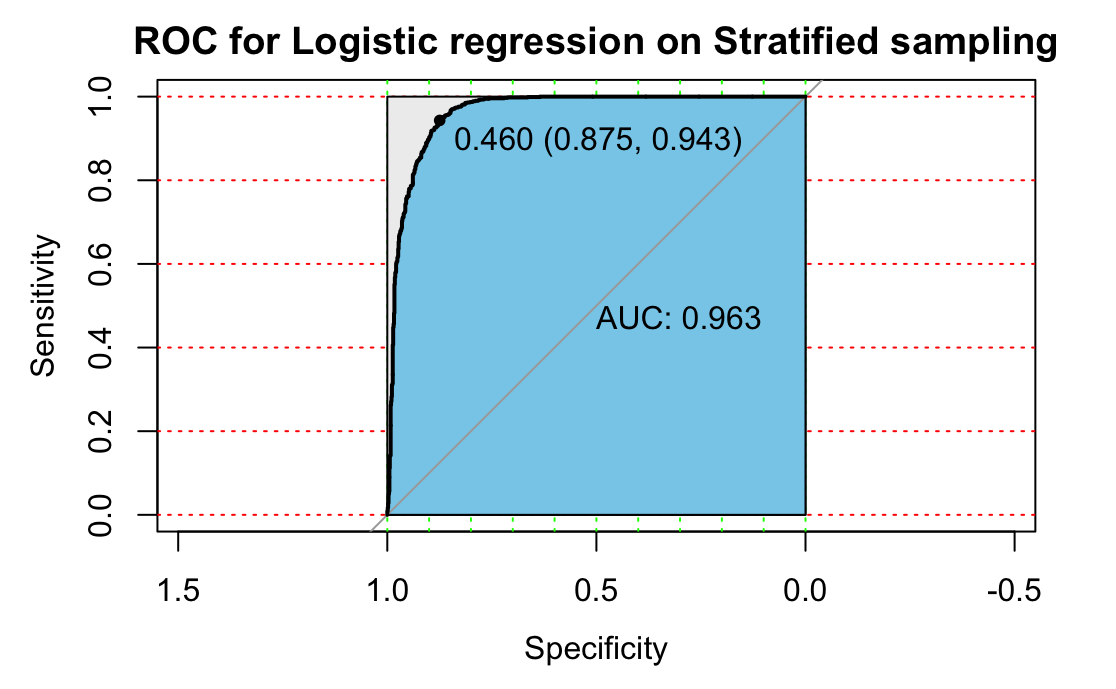
\includegraphics[width=1\textwidth, height=0.65\textwidth]{../figures/ROC_LR_s.png}
  \end{subfigure}%
  \caption{ROC of Logistic Regression}
\end{figure}
\item The test set ROC of the decision tree model in random sampling samples and stratified sampling samples are as follows:
\begin{figure}[H]
  \centering
  \begin{subfigure}{.5\textwidth}
    \centering
      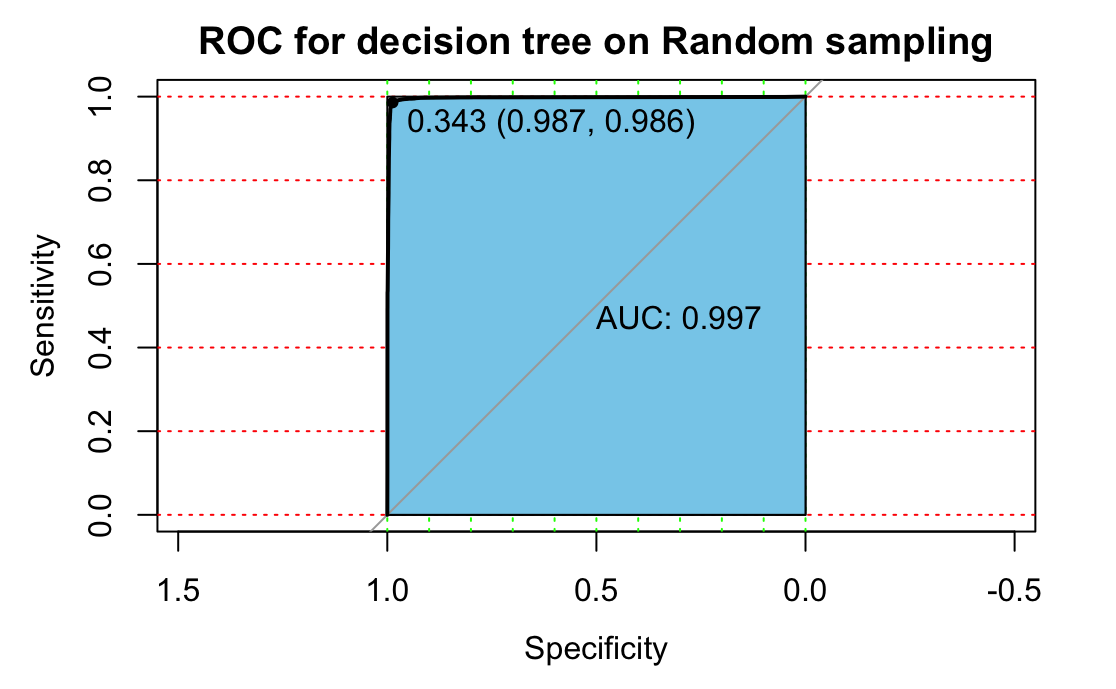
\includegraphics[width=1\textwidth, height=0.65\textwidth]{../figures/ROC_DT_random.png}    
  \end{subfigure}%  
  \begin{subfigure}{.5\textwidth}
    \centering
      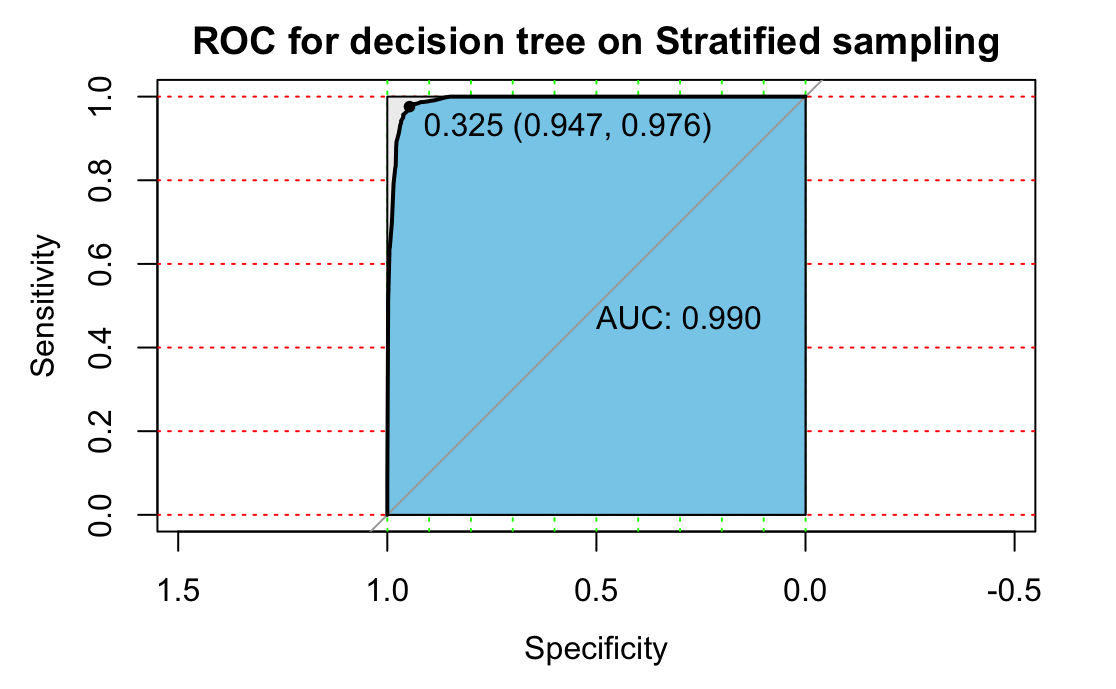
\includegraphics[width=1\textwidth, height=0.65\textwidth]{../figures/ROC_DT_s.png}
  \end{subfigure}%
  \caption{ROC of Decision Tree}
\end{figure}
\item The test set ROC of the random forest model in random sampling samples and stratified sampling samples are as follows:
\begin{figure}[H]
  \centering
  \begin{subfigure}{.5\textwidth}
    \centering
      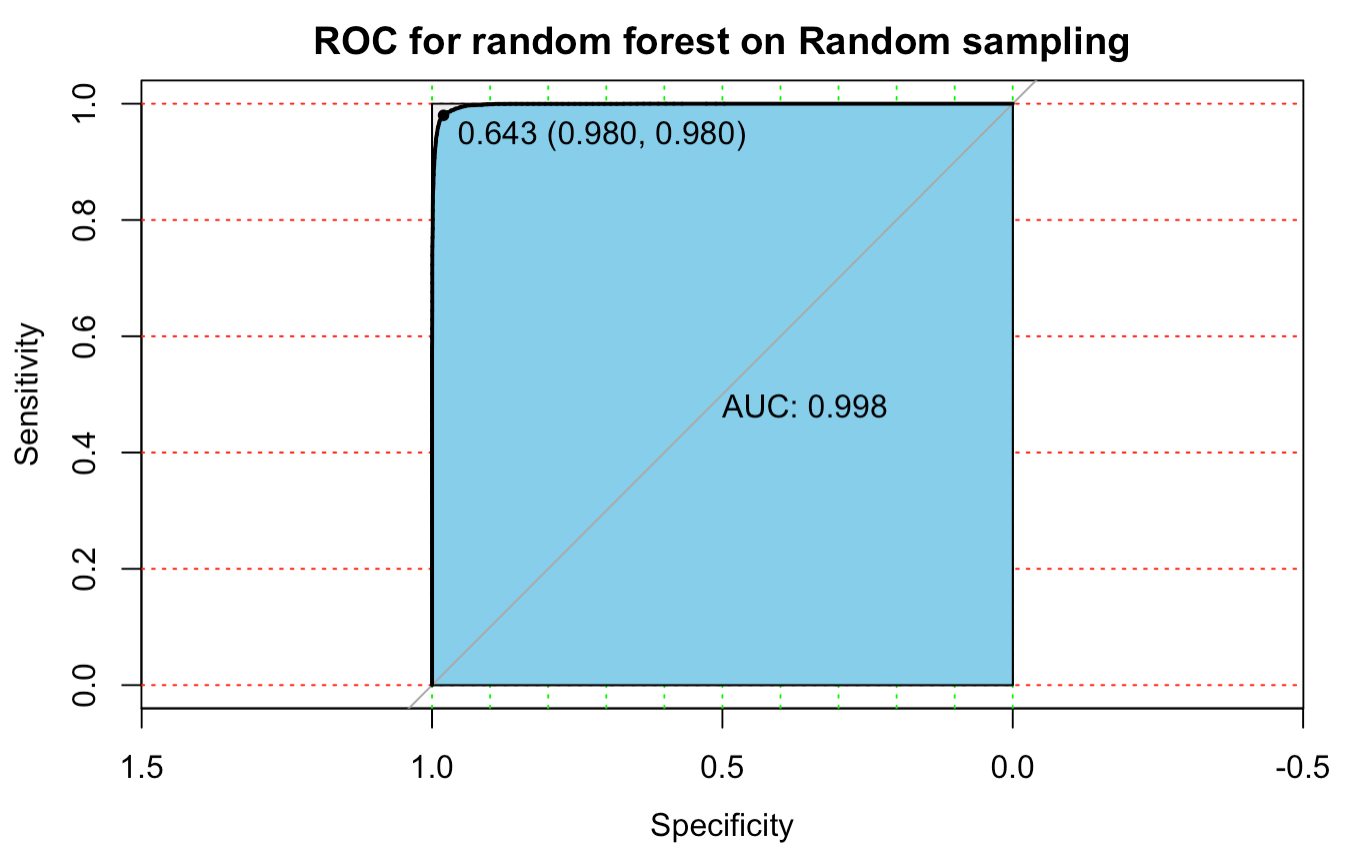
\includegraphics[width=1\textwidth, height=0.65\textwidth]{../figures/ROC_RF_random.png}    
  \end{subfigure}%  
  \begin{subfigure}{.5\textwidth}
    \centering
      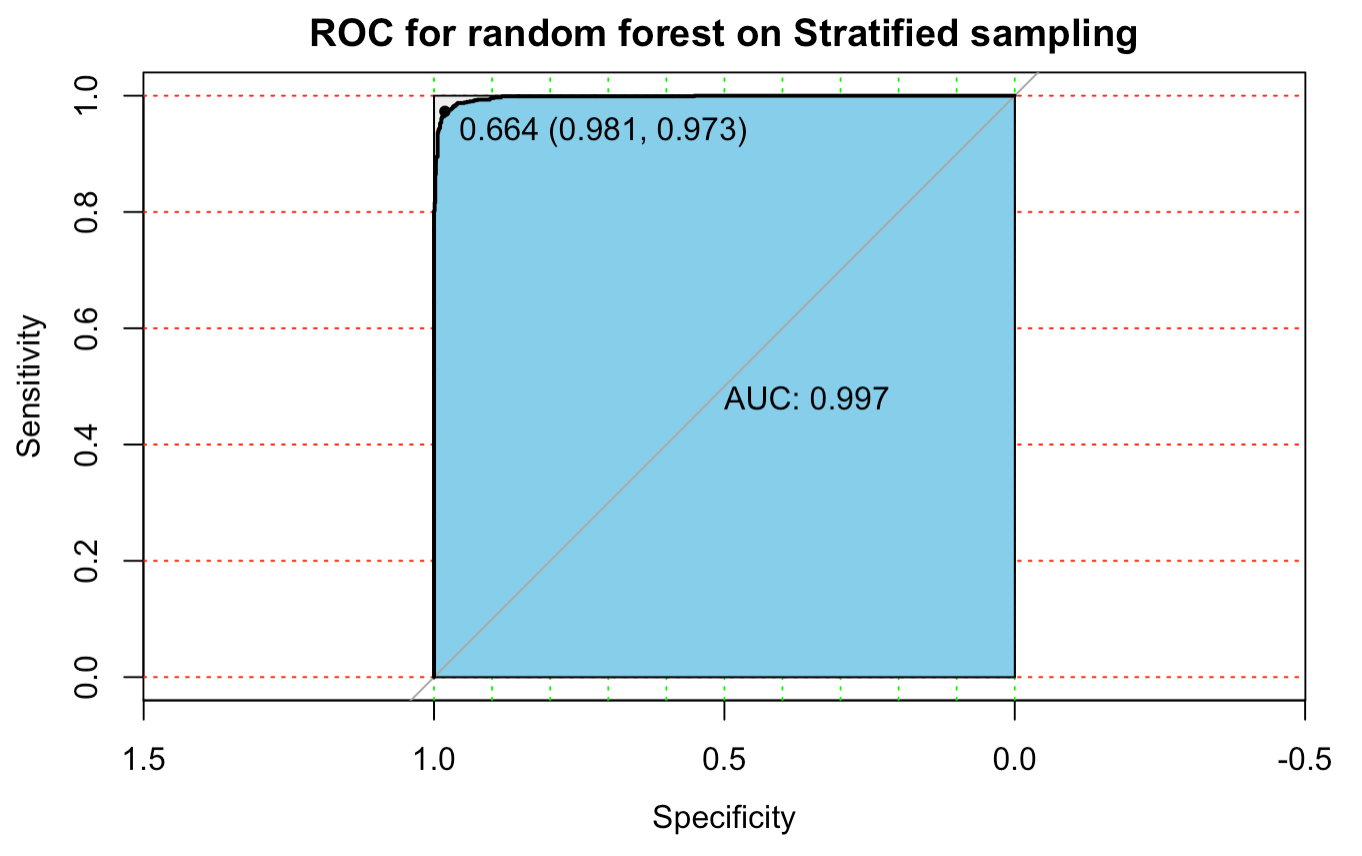
\includegraphics[width=1\textwidth, height=0.65\textwidth]{../figures/ROC_RF_s.png}
  \end{subfigure}%
  \caption{ROC of Random Forest}
\end{figure}
\item The test set ROC of SVM in random sampling samples and stratified sampling samples are as follows:
\begin{figure}[H]
  \centering
  \begin{subfigure}{.5\textwidth}
    \centering
      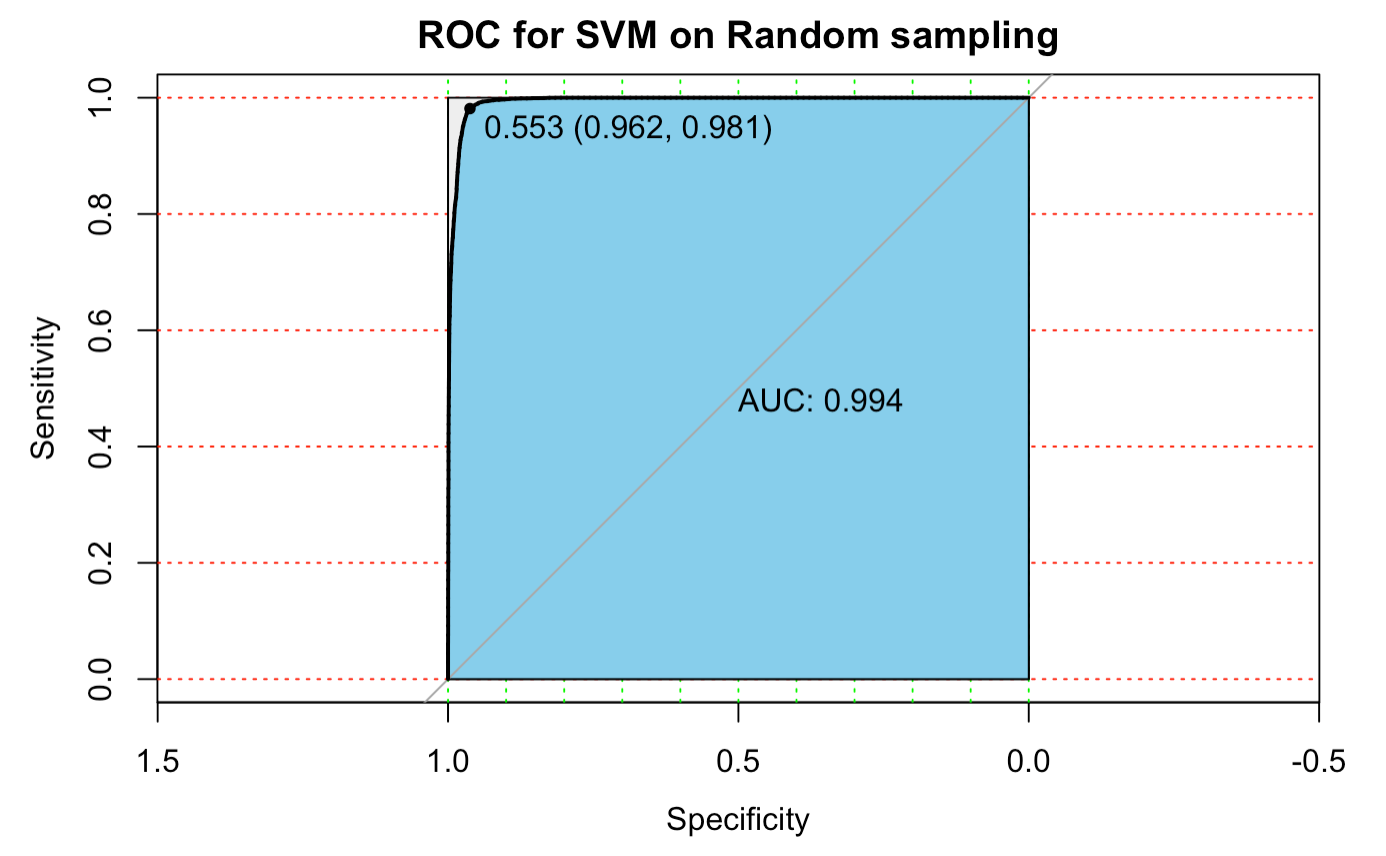
\includegraphics[width=1\textwidth, height=0.65\textwidth]{../figures/ROC_SVM_random.png}    
  \end{subfigure}%  
  \begin{subfigure}{.5\textwidth}
    \centering
      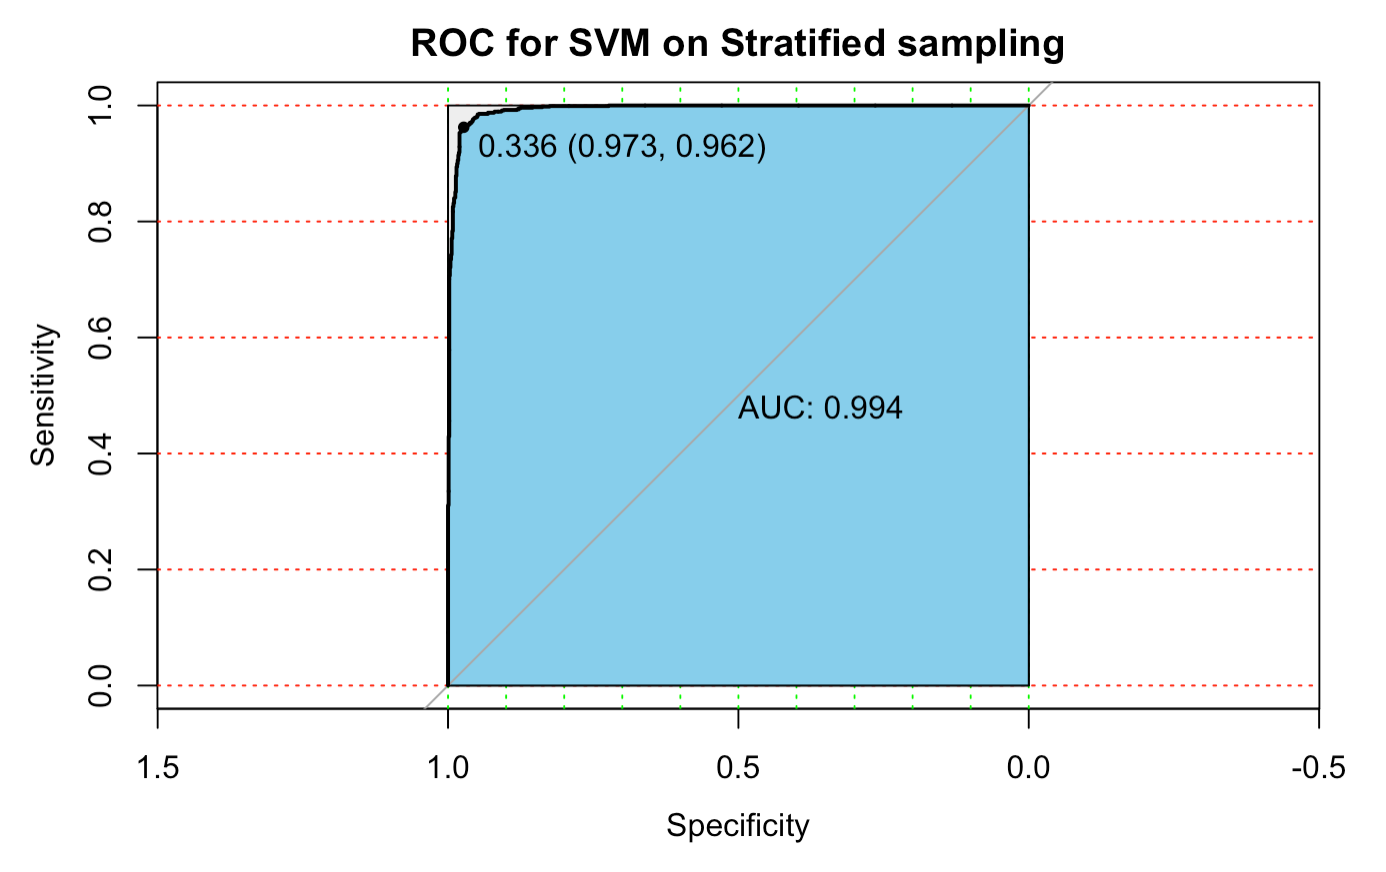
\includegraphics[width=1\textwidth, height=0.65\textwidth]{../figures/ROC_SVM_s.png}
  \end{subfigure}%
  \caption{ROC of SVM}
\end{figure}
\end{itemize}

The performance of the four models in the cross-validation is very close to the test set, and no underfitting and overfitting problems were found. Comparing the classification accuracy and AUC value of the four models in the test set, it can be found that random forest is the best. And using randomly sampled samples as the training set, the performance of random forest will be better.

\begin{table}[htbp]
\centering
	\begin{tabular}{|c|c|c|c|}  
		\hline  
		& &  \\[-8pt]  
		Testing AUC&Random sampling&Stratified sampling \\ 
		\hline
		& &  \\[-8pt] 
		Logistic Regression&0.9582 &0.9630  \\
		\hline
		& &  \\[-8pt] 
		Decision Tree&0.9911 &0.9913  \\
		\hline
		& &  \\[-8pt] 
		Random Forest&0.9981 &0.9972 \\
		\hline
		& &  \\[-8pt] 
		SVM	&0.9937 &0.9936  \\
		\hline
	\end{tabular}
\end{table}

\section{Diagnostics}

\quad\ \ According to the previous analysis, I feel that random forest is chosen as the final prediction model. For the optimal random forest, we think that 60 trees are enough. The figure below shows the relationship between the number of trees in the forest and the model error. When the number of decision trees increases to about 50, the error of the random forest reaches convergence.

\begin{figure}[H]
  \centering
      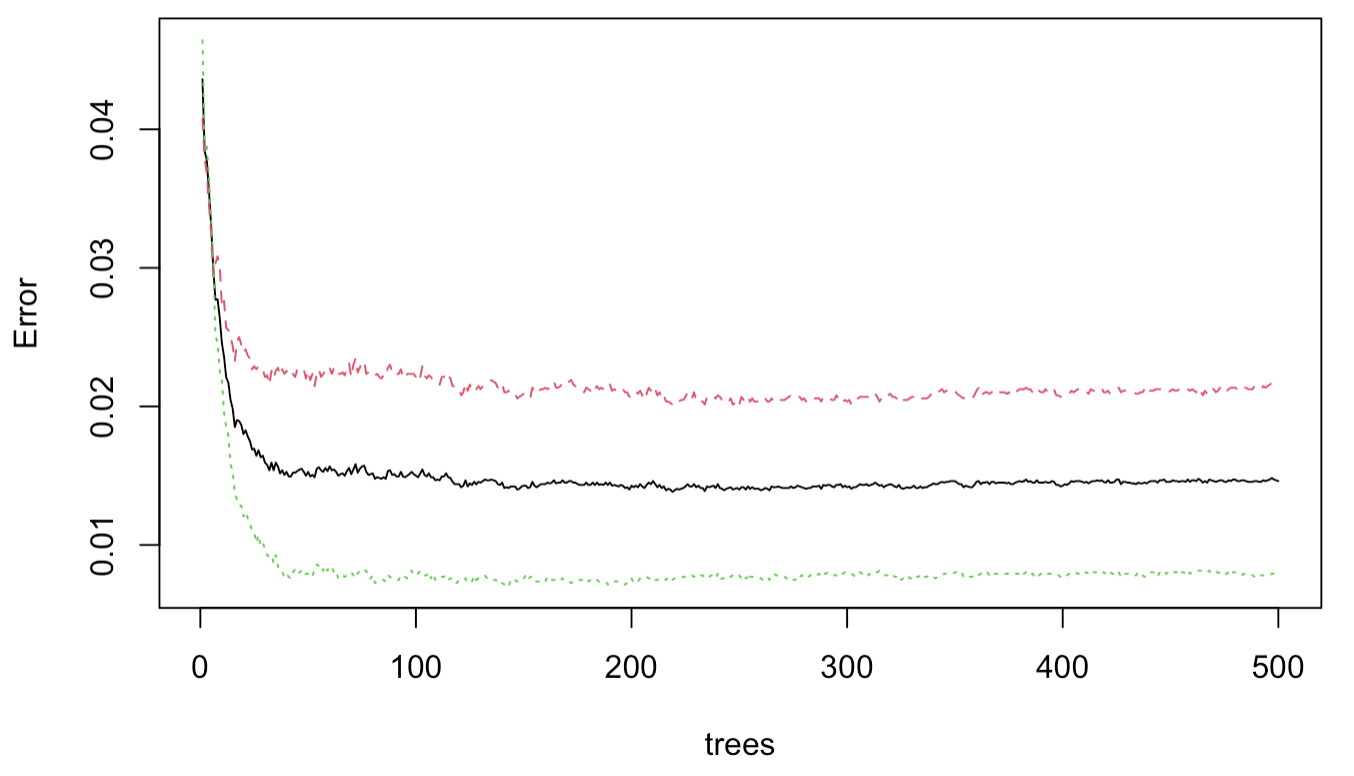
\includegraphics[width=0.85\textwidth, height=0.45\textwidth]{../figures/RF.png}    
  \caption{Error of Random Forest}
\end{figure}

The feature importance of random forest is shown in the figure below. \textbf{NDAI} is the most important, followed by location coordinates, and radiance-related features are relatively unimportant.

\begin{figure}[H]
  \centering
      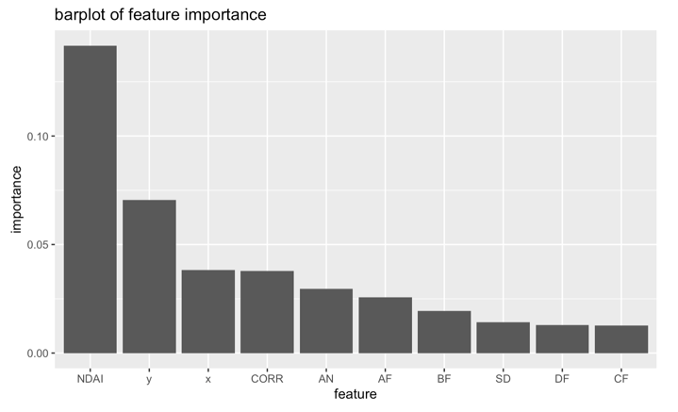
\includegraphics[width=0.85\textwidth, height=0.45\textwidth]{../figures/barplot.png}    
  \caption{Feature Importance of Random Forest}
\end{figure}

\newpage
Draw the edge of the predictor from the random forest classifier. From the margin graph, even if it is distributed in the edge of the image, the prediction performance of the random forest will hardly change. It means that the model has very strong robustness.

\begin{figure}[H]
  \centering
      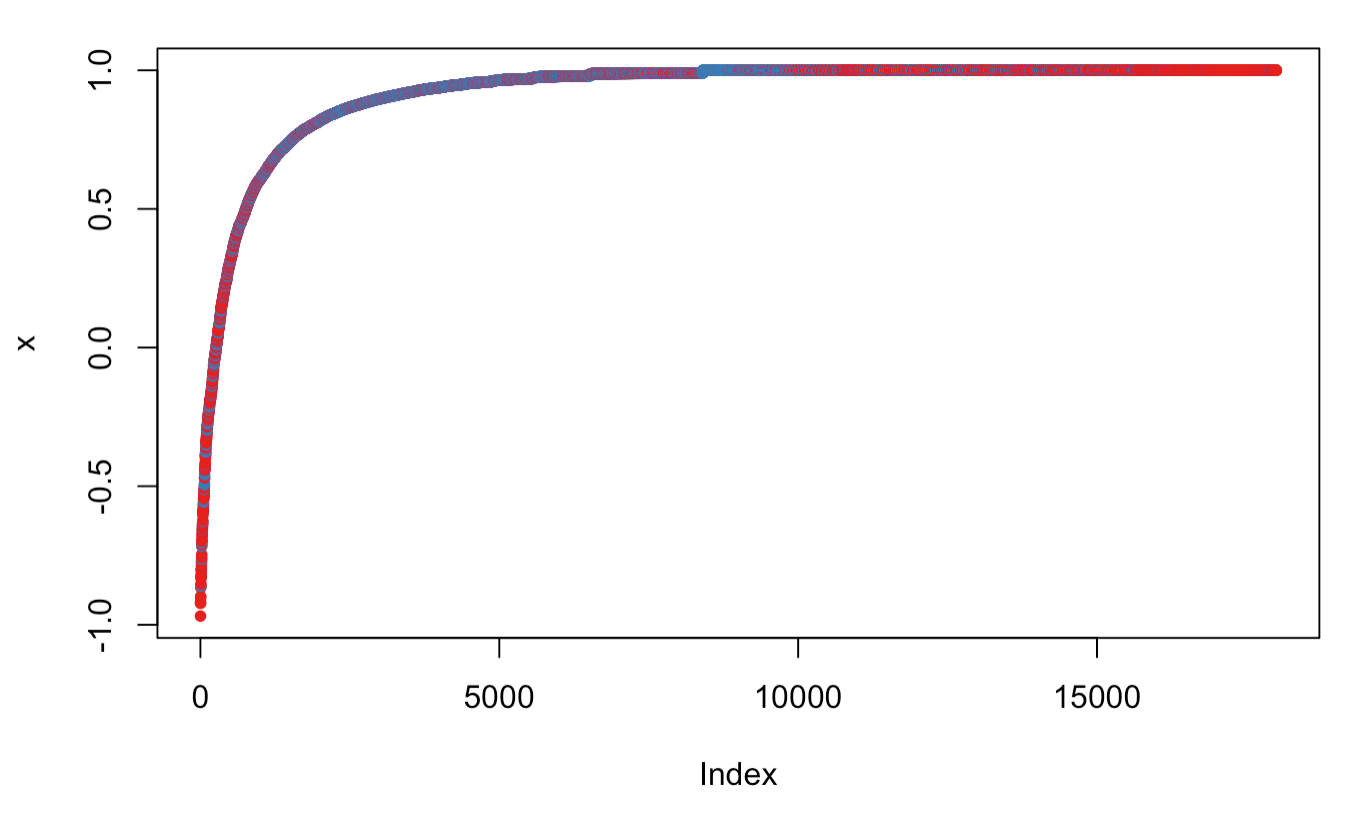
\includegraphics[width=0.85\textwidth, height=0.45\textwidth]{../figures/edge_RF.png}    
  \caption{Edge of Predictor from Random Forest Classifier}
\end{figure}

The following is the confusion matrix of the random forest. For the cases of expert labels, the random forest classification error rate is $0.821\%$. Random forest seems to be better at predicting cloud cases, but relatively weaker for 

\begin{figure}[H]
  \centering
      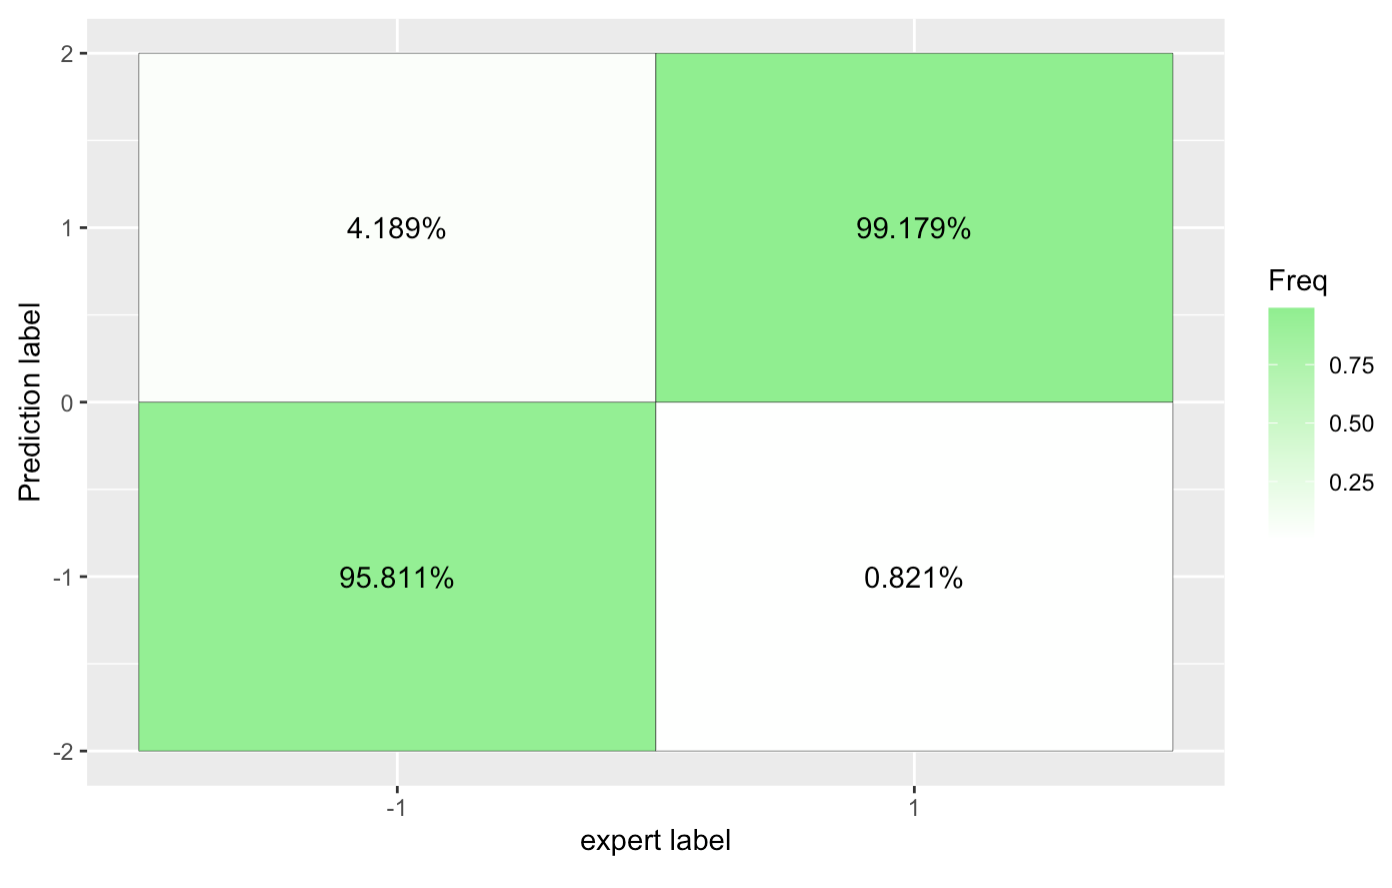
\includegraphics[width=0.85\textwidth, height=0.45\textwidth]{../figures/matrix.png}    
  \caption{Confusion Matrix of Random Forest}
\end{figure}

In the exploratory analysis, we can find that the characteristic distribution of different weathers is different through visualization and correlation analysis, and there is a significant correlation between the characteristic variables. We consider all the characteristic variables as model inputs. We first standardize the data, and use random sampling and stratified sampling to construct training, verification, and test sets. For each sampling method, we build 4 models: logistic regression, decision tree, random forest, and SVM. For each model, use 5-fold cross-validation to calculate the classification accuracy of each fold and the classification accuracy and AUC on the test set. After model performance comparison, it is found that the random forest constructed by dividing the data set by random sampling method is the best, with an average cross-validation classification accuracy rate of 0.9784 and a test set AUC of 0.9981. Random forest is very robust, and it also has a very high classification accuracy for samples distributed on the margin.

\bigskip

\center{\textit{Reference}}

Tao SHI, Bin YU, Eugene E. CLOTHIAUX, and Amy J. BRAVERMAN,"Daytime Arctic Cloud Detection Based on Multi-Angle Satellite Data With Case Studies", 2008.



\bibliographystyle{plain}
\bibliography{report}
\end{document}
